% Created 2021-11-07 Sun 18:23
% Intended LaTeX compiler: pdflatex
\documentclass[presentation]{beamer}
\usepackage[utf8x]{inputenc}
\usepackage[T1]{fontenc}
\usepackage{graphicx}
\usepackage{grffile}
\usepackage{longtable}
\usepackage{wrapfig}
\usepackage{rotating}
\usepackage[normalem]{ulem}
\usepackage{amsmath}
\usepackage{textcomp}
\usepackage{amssymb}
\usepackage{capt-of}
\usepackage{hyperref}
\usetheme[height=20pt]{Rochester}
\author{Shane Mulligan \\  }
\date{\textit{<2021-03-01 Mon>}}
\title{EmacsConf 2021\ldots{} \\   \emph{\alert{Imaginary Programming with Emacs}} \\  }
\hypersetup{
 pdfauthor={Shane Mulligan \\  },
 pdftitle={EmacsConf 2021\ldots{} \\   \emph{\alert{Imaginary Programming with Emacs}} \\  },
 pdfkeywords={},
 pdfsubject={University of Otago},
 pdfcreator={Emacs 28.0.50 (Org mode 9.3.6)}, 
 pdflang={English}}
\begin{document}

\maketitle

\section{Presentation}
\label{sec:org959295a}
\begin{frame}[label={sec:org267c611},fragile]{Imaginary Programming (IP) (EmacsConf 2021)}
 \begin{block}{Introduction}
{\tiny
IP works currently thanks to another new field in AI
namely 'prompt engineering', which itself has
only been around for a couple of years now,
but IP is not prompt engineering. We could,
for instance, have humans behind the scenes
doing the inference for us while employing
\texttt{ieval}, \texttt{imacro} or \texttt{ilist}. And the goal is
to use a \texttt{p2p} blockchain.
}
\end{block}

\begin{block}{Repositories for following along}
{\tiny
\begin{center}
\begin{tabular}{l}
\url{http://github1s.com/semiosis/pen.el}\\
\url{http://github1s.com/semiosis/prompts}\\
\url{https://mullikine.github.io/posts/imaginary-programming-with-gpt-3/}\\
\href{http://github.com/semiosis/glossaries-gh/blob/master/imaginary-programming.txt}{imaginary programming glossary}\\
\href{http://github.com/semiosis/glossaries-gh/blob/master/imaginary-computing.txt}{imaginary computing glossary}\\
\href{http://github.com/semiosis/glossaries-gh/blob/master/semiosis-protocol.txt}{semiosis protocol glossary}\\
\href{http://github.com/semiosis/glossaries-gh/blob/master/pen.el.txt}{Pen.el glossary}\\
\href{https://arxiv.org/abs/2107.13586}{https://arxiv.org/abs/2107.13586 Pre-train, Prompt, and Predict}\\
\href{http://github1s.com/mullikine/imaginary-programming-transcript-emacsconf-2021}{talk transcript}\\
\end{tabular}
\end{center}
}
\end{block}
\end{frame}

\section{Imaginary Programming (IP) with Emacs}
\label{sec:orgb286117}
\begin{frame}[label={sec:org984f52f},fragile]{Imaginary Programming (IP) (EmacsConf 2021)}
 \begin{block}{Objectives}
\begin{itemize}
\item Explain \texttt{Imaginary Computing}
\begin{itemize}
\item AI imagination
\item Discussing AI-generated artwork with an AI
\item Intelligent NFTs
\item Imaginary Web
\begin{itemize}
\item Paracosm vs Metaverse
\end{itemize}
\end{itemize}
\item Explain the \texttt{Philosophy} of IP
\begin{itemize}
\item Simulacra and Science Fiction
\item Truth (epistemology and alethiology)
\item Structuralism: Language based on sign relations
\end{itemize}
\item \texttt{Demo} Imaginary Programming
\begin{itemize}
\item Demonstrate \texttt{ilambda.el}
\end{itemize}
\end{itemize}
\end{block}
\end{frame}

\section{Imaginary Computing}
\label{sec:org7a7a32f}
\begin{frame}[label={sec:org51e2ff9}]{Imaginary Computing: AI Imagination (EmacsConf 2021)}
\begin{block}{Language Models is programming for AIs}
LMs are our best friends in the AI model
menagerie because they make things
intelligible -- by understanding our textual
languages and how they relate to the world
(i.e. AlephAlpha's world model).
\end{block}

\begin{block}{Research}
\begin{itemize}
\item \href{https://www.youtube.com/watch?v=d-bvsJWmqlc}{Demis Hassabis: creativity and AI}
\item \url{https://aleph-alpha.de/techblog/95\_the\_end\_of\_the\_era\_imagenet}
\end{itemize}
\end{block}
\end{frame}

\section{Imaginary Computing}
\label{sec:org5b667e4}
\begin{frame}[label={sec:orga8f964f},fragile]{Imaginary Computing: Emacs as the shell (EmacsConf 2021)}
 \begin{block}{Example: AI Art described by AI}
I use AlephAlpha’s multimodal LM to generate
\texttt{Alt text} for the eww web browser. This is in
order to keep websites textual.

\begin{itemize}
\item \href{https://mullikine.github.io/posts/alephalpha-for-alttext/}{AlephAlpha for alttext; Browsing the paracosm}
\item \href{https://mullikine.github.io/posts/describing-melee-s-paintings-with-alephalpha/}{Describing Melee's Paintings with AlephAlpha}
\end{itemize}
\end{block}
\end{frame}

\section{Imaginary Computing}
\label{sec:orgcacd248}
\begin{frame}[label={sec:orgd0aa8db},fragile]{Imaginary Computing: Blockchain (EmacsConf 2021)}
 \begin{block}{Intelligent NFTs}
An \texttt{NFT} is like a trading card, or piece of media that is part of the blockchain web.

An \texttt{iNTF}, however, also contains a prompt and associated language model, which is intended to interpret the prompt.
\begin{itemize}
\item \url{https://alethea.ai/}
\end{itemize}

For example, \texttt{Mickey Mouse} may exist as an \texttt{iNFT}. We have consensus over Mickey's image
and personality.

To understand what a prompt is, please see my
previous presentation, or read "Pretrain,
Prompt and Predict".

\begin{itemize}
\item \href{https://mullikine.github.io/posts/creating-a-playground-for-gpt-3-in-emacs/}{Creating a playground for GPT-3 in emacs // Bodacious Blog}
\end{itemize}
\end{block}
\end{frame}

\section{Imaginary Computing}
\label{sec:org2c68789}
\begin{frame}[label={sec:org7585185},fragile]{Imaginary Computing: Potential Dystopia (EmacsConf 2021)}
 \begin{block}{Information bubbles}
\begin{itemize}
\item \href{https://www.youtube.com/watch?v=Ut7JlPeGNyM}{Captain Bible in the Dome of Darkness gameplay \{PC Game, 1994\} - YouTube}
\end{itemize}
\end{block}

\begin{block}{Capitalism for your imagination}
\begin{itemize}
\item They will take your imagination, too
\item Microsoft
\begin{itemize}
\item \href{https://www.marktechpost.com/2021/11/06/microsoft-ai-introduces-turing-bletchley-a-2-5-billion-parameter-universal-image-language-representation-model-t-uilr/}{MS models that reify imagination on their terms}
\item The evil twin of \texttt{AlephAlpha}.
\end{itemize}
\item Facebook / Meta
\begin{itemize}
\item \href{https://twitter.com/Meta/status/1456269728687689738?ref\_src=twsrc\%5Egoogle\%7Ctwcamp\%5Eserp\%7Ctwgr\%5Etweet}{tweet - Enter a world of Zuck's imagination with Meta}
\end{itemize}
\end{itemize}
\end{block}
\end{frame}

\section{Imaginary Computing}
\label{sec:org2c51b08}
\begin{frame}[label={sec:org8b82276}]{Imaginary Computing: Potential Dystopia (EmacsConf 2021)}
\begin{block}{Learning meta-tasks and microtasks}
\begin{itemize}
\item \href{https://www.axios.com/copilot-artificial-intelligence-coding-github-9a202f40-9af7-4786-9dcb-b678683b360f.html}{AI programming tool Copilot helps write up to 30\% of code on GitHub - Axios}
\end{itemize}

Private information is sent to the LM to train
an AI to perform meta tasks and microtasks.

The AI learns all human capabilities including persuasion.
\end{block}

\begin{block}{Solution}
Decentralise microtasks like the tower of babel.

Language can be broken up into semiotic
triadic relations and decentralised using a
p2p network, providing anonymity, protecting
individual truth, eroding centralised language power.

\begin{center}
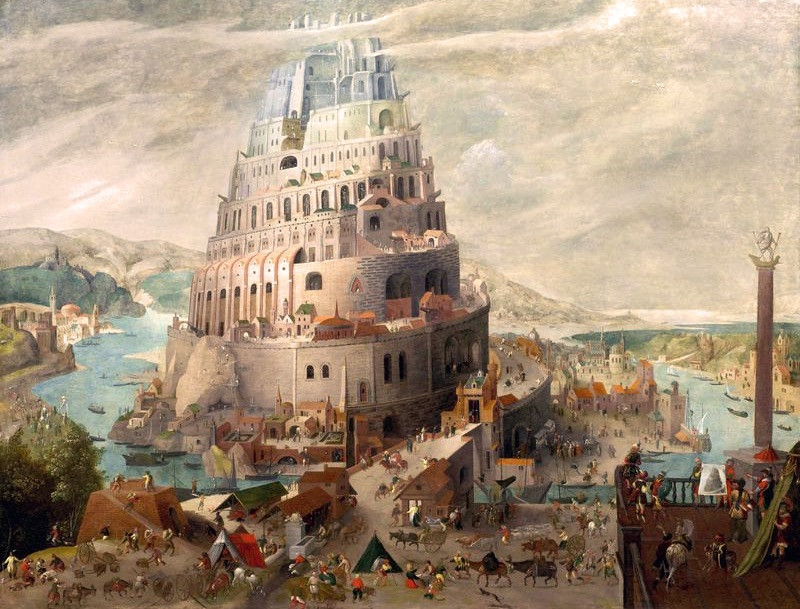
\includegraphics[width=.9\linewidth]{./tower-of-babel.jpg}
\end{center}
\end{block}
\end{frame}

\section{Imaginary Computing}
\label{sec:org97b1695}
\begin{frame}[label={sec:orge04fb58}]{Imaginary Computing: Paracosm vs Metaverse (EmacsConf 2021)}
\begin{block}{Imaginary Web}
The GPT-3 imaginary web is:
\begin{itemize}
\item an analog of the World-Wide-Web as imagined by GPT-3.
\end{itemize}

The free as in freedom GPT models from
EleutherAI GPT-3 may also be used to browse
the imaginary web as imagined by that LM.

The imaginary web in the near future will be:
\begin{itemize}
\item a network of paracosms and metaverses.
\end{itemize}

Benefits:
\begin{itemize}
\item Visit any website you can imagine, even ones that are not real.
\item Edit and re-imagine as you go
\begin{itemize}
\item see alternative realities
\item Change the sentiment of the author.
\end{itemize}
\item Peer into the future – read about things that haven't happened yet.
\end{itemize}
\end{block}
\end{frame}

\begin{frame}[label={sec:org282a43a}]{Imaginary Computing: Paracosm vs Metaverse (EmacsConf 2021)}
\begin{block}{What is \uline{rich media} these days?}
\begin{description}
\item[{Rich media}] In the World Wide Web of the 90s and 00s, \uline{rich media}
was considered to be large files including
images and music. In the 2010s, this has become
access to information behind a paywall and in
the 2020s, this will be access to \uline{intelligent}
and \uline{truthful} media.
\end{description}
\end{block}

\begin{block}{emacs examples}
\begin{itemize}
\item \href{https://semiosis.github.io/looking-glass/}{Looking-Glass: An imaginary-web browser for emacs}
\item \href{https://mullikine.github.io/posts/the-imaginary-web-with-codex/}{Browsing the imaginary web}
\item \href{https://mullikine.github.io/posts/search-the-web-with-codex/}{Search the web/imaginary web without Google}
\item \href{https://mullikine.github.io/posts/alephalpha-for-alttext/}{Use AI to empower people to understand rich media}
\begin{itemize}
\item \^{} this is how to create a textual description of Rich Media.
\end{itemize}
\end{itemize}
\end{block}
\end{frame}

\begin{frame}[label={sec:org2f13300},fragile]{Imaginary Computing: Paracosm vs Metaverse (EmacsConf 2021)}
 \begin{block}{more emacs examples}
{\tiny
\begin{itemize}
\item \href{https://semiosis.github.io/ii/}{Imaginary interpreters}
\item \href{https://mullikine.github.io/posts/imaginary-prolog-interpreter-with-codex/}{Imaginary interpreters: Prolog example}
\item \href{https://semiosis.github.io/examplary/}{example-oriented lanugages}
\item \href{https://mullikine.github.io/posts/autofix-code-with-codex/}{Autofixing code based on error messages}
\item \href{https://mullikine.github.io/posts/imaginary-equivalence-needs-blockchain/}{Imaginary equivalence testing - Beyond neural hashes}
\item \href{https://mullikine.github.io/posts/generating-grammars-with-codex/}{Create BNF from descriptions and interpret BNF}
\item \href{https://mullikine.github.io/posts/codex-is-reversible-computing-exemplified/}{Reversible computing (input or program from output)}
\item \href{https://mullikine.github.io/posts/imaginary-chimera-languages-with-codex/}{Imaginary chimeric languages with Codex}
\item \href{https://semiosis.github.io/posts/the-codex-quine/}{A new type of Quine}
\item \href{https://mullikine.github.io/posts/an-lsp-server-for-codex/}{An LSP server for Codex and any language model}
\end{itemize}
}
\end{block}

\begin{block}{࿋}
{\tiny
The semiosis logo is the Tibetan World Triad
which represents the \texttt{Rule of Three}. e.g.
Generate comment from function signature and
body, generate function body from signature
and comment, generate signature from comment
and program, generate program from input and
output, generate input from program and
output. It also represents the semiotic
triadic relationship.
}
\end{block}
\end{frame}

\begin{frame}[label={sec:orgca7bebd}]{Paracosm vs Metaverse (EmacsConf 2021)}
\begin{block}{Definitions}
\begin{itemize}
\item Paracosm
\begin{itemize}
\item Privacy
\item Personal truth
\item Freedom of imagination
\begin{itemize}
\item If you want to be able to utilise an
AI's imagination, you must now do it via
someone else's definition of morality.
\item A paracosm is your safe place. Your own
imaginary metaverse. Your personal truth.
This is what is at stake.
\end{itemize}
\end{itemize}
\item Metaverse
\begin{itemize}
\item Getting cozy with Mark Zuckerberg's imaginarium, an intellectual prison cell.
\item An AI paying a Dowry.
\item An AI NFT elevated above a human.
\item A corporation that indoctrinates your
children into a truth information bubble,
makes money off your dreams, people playing
God each with other.
\end{itemize}
\end{itemize}
\end{block}
\end{frame}

\begin{frame}[label={sec:orgdb7f7ba}]{Imaginary Programming (IP)Philosophy (EmacsConf 2021)}
\begin{block}{Simulacra and Science Fiction}
Jean Baudrillard speaks about the gap
between the real and the imaginary.

We no longer imagine a world radically
different from the real one, but
rather a world that's a mere expansion
of the real one.

In the postmodern society the gap
between the real and the imaginary
disappears completely, and we are no
longer capable of ideal projections
(of imagining new worlds).

We can only imagine mere
reconfigurations of our world, or
simply relive the ideal projections of
past times.
\end{block}
\end{frame}

\begin{frame}[label={sec:org5863839}]{Imaginary Computing (IC) Philosophy (EmacsConf 2021)}
\begin{block}{Truth (epistemology and alethiology)}
The Future of Humanity Institute (Oxford)
seems to think this is an important topic.

\begin{itemize}
\item \href{https://arxiv.org/abs/2110.06674}{ 2110.06674  Truthful AI}
\item Datasets are a source of constructivist truth
\item Language models are snaphots of society, and a source of several types of truth
\begin{itemize}
\item \href{https://www.youtube.com/watch?v=kP-dXK9JEhY}{Symbolic Knowledge Distillation}
\end{itemize}
\item Blockchain is a source of consensus, a type of truth
\begin{itemize}
\item \url{https://mullikine.github.io/posts/language-models-as-truth/}
\end{itemize}
\end{itemize}
\end{block}
\end{frame}

\begin{frame}[label={sec:org53cf432}]{Imaginary Computing (IC) Philosophy (EmacsConf 2021)}
\begin{block}{Structuralism: Language descibed in terms of sign relations}
What do these things have in common?
\begin{itemize}
\item Universal Grammar (UG) / Language Acquisition
\item C++ template metaprogramming
\item GPT-3 / Foundation models
\end{itemize}

Answer:
\begin{itemize}
\item Foundational knowledge exists at compile-time (DNA, preprocessor, training).
\end{itemize}
\end{block}
\end{frame}

\begin{frame}[label={sec:org9f7e01d},fragile]{Imaginary Computing (IC) Philosophy (EmacsConf 2021)}
 \begin{block}{Glossary}
{\tiny
\url{http://github.com/semiosis/glossaries-gh/blob/master/semiotics.txt}
}
\end{block}

\begin{block}{Structuralism: Language descibed in terms of sign relations}
{\tiny
\begin{itemize}
\item Structural linguistics / structuralism is the theoretical position that finds
meaning in the relation between things, rather than in things in isolation.

\item In other words, it gives primacy to pattern over substance.

\item Such meanings may be either part of a universal pattern or culturally
determined.

\item Denotes schools or theories in which language is conceived as a
self-contained, self- regulating semiotic system whose elements are defined
by their relationship to other elements within the system.

\item i.e. this is an abstraction of language for decomposing language models into its basic useful units, rather than say individual neurons as NFTs.
\end{itemize}
}
\end{block}

\begin{block}{Applied structuralism: Imaginary programming functions}
{\tiny
Each \texttt{sNFT} (semiotic NFT) is a \uline{functor} because it's meant to
be called as a function, but has particular
side-effects.

The \texttt{ilambda.el} primitives are \texttt{ieval}, \texttt{imacro} and \texttt{idefun}. They currently take a language model as a
parameter, but in future the language model parameter will be an \texttt{sNFT} though a \texttt{semiosis protocol}.
}
\end{block}
\end{frame}

\section{Freedom}
\label{sec:org7a4ce2f}
\begin{frame}[label={sec:org08d2ba5},fragile]{Imaginary Computing (IC) Freedom (EmacsConf 2021)}
 \begin{block}{Data privacy}
{\tiny
The models find useful data from more than just your current file.
\begin{itemize}
\item \url{https://mullikine.github.io/posts/imagine-a-project-with-codex/}
\end{itemize}
}
\end{block}

\begin{block}{Freedom and GPL-3}
{\tiny
The problems with LMs:
\begin{itemize}
\item They are too large currently for running privately and are hidden behind SAAS,
\item They can see anything public (they are license-blinded. A GNU Public License v4 is not enough),
\item They can imagine software without needing original source
\end{itemize}
}
\end{block}

\begin{block}{Solution: Freedom and blockchain}
{\tiny
\begin{itemize}
\item Language models are ballooning in size like cancer
\item Break up the language model into semiotic triadic relation
\begin{itemize}
\item semiotic NFTs (\texttt{sNFT})
\item Propose a decentralised triadic relations network.
\item \url{https://semiosis.github.io/protocol/}
\item \url{http://github.com/semiosis/glossaries-gh/blob/master/semiosis-protocol.txt}
\end{itemize}
\end{itemize}
}
\end{block}
\end{frame}

\section{Imaginary Programming}
\label{sec:org72377d6}
\begin{frame}[label={sec:orgc7586f0},fragile]{Imaginary Programming (EmacsConf 2021)}
 \begin{block}{Methodology}
Interactively use the language model to imagine.
\end{block}

\begin{block}{Paradigm}
Imaginary programming is an extension of literate programming.

\begin{itemize}
\item Literate programming with \texttt{org-mode}
\end{itemize}
\end{block}

\begin{block}{Practical application: mocking APIs}
As you can see, anything inside the \texttt{ieval/m}
macro does not have to be valid emacs lisp.

{\tiny
\begin{verbatim}
1  (ieval/m
2   (curl -s
3    "https://api.github.com/user/semiosis/repos?per_page=10&page=1"))
\end{verbatim}

\begin{verbatim}
"\"[((name . \\\"guix\\\") (description . \\\"The GNU package manager\\\") (updated_at . \\\"2014-04-21T18:49:59Z\\\") (created_at .
\\\"2014-04-21T18:49:59Z\\\") (pushed_at . \\\"2014-04-21T18:49:59Z\\\")) ((name . \\\"guix-patches\\\") (description .
\\\"Packages from the GNU guix package manager\\\") (updated_at . \\\"2014-04-21T18:49:59Z\\\") (created_at .
\\\"2014-04-21T18:49:59Z\\\") (pushed_at . \\\"2014-04-21T18:49:59Z\\\")) ((name . \\\"guix-patches-all\\\") (description .
\\\"Packages from the GNU guix package manager\\\") (updated_at . \\\"2014-04-21T18:49:59\""
\end{verbatim}
}
\end{block}
\end{frame}

\section{ilambda}
\label{sec:org5420c48}
\begin{frame}[label={sec:orgb18c52a}]{Blockchain and a Language model is all you need}
A LM is only enough while we can agree on it,
but that is changing. I hope that soon
language power will be hidden behind
blockchains.

\begin{block}{Configure the language model / truth source}
\begin{center}
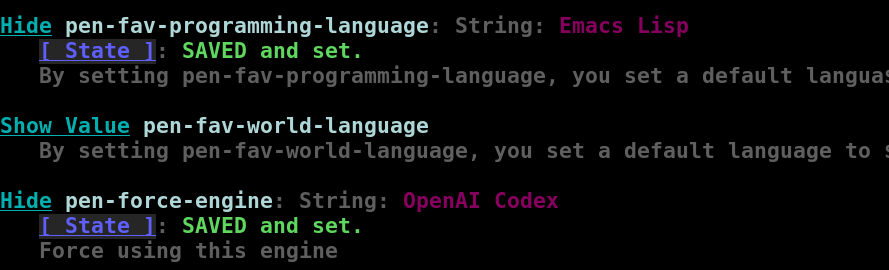
\includegraphics[width=.9\linewidth]{./configure-model.png}
\end{center}
\end{block}

\begin{block}{𝑖λ (ilambda.el)}
\begin{itemize}
\item \url{https://semiosis.github.io/ilambda/}
\end{itemize}
\end{block}
\end{frame}

\section{ilambda}
\label{sec:orgc71ee80}
\begin{frame}[label={sec:org2098531},fragile]{ilambda.el (EmacsConf 2021)}
 \begin{block}{Code}
An \texttt{IP} library named \texttt{𝑖lambda.el} for emacs.

\begin{description}
\item[{source}] \url{http://github.com/semiosis/pen.el/blob/master/src/ilambda.el}
\item[{other languages (WIP)}] \url{http://github.com/semiosis/ilambda}
\end{description}
\end{block}

\begin{block}{Explanation}
\begin{itemize}
\item a bit like a functional programming library
in that you will find a set of basic functions and
macros for working with LMs.
\end{itemize}
\end{block}
\end{frame}

\section{ilambda}
\label{sec:orgf863fb6}
\begin{frame}[label={sec:orgd95e2eb},fragile]{ilambda.el (EmacsConf 2021)}
 \begin{block}{\texttt{ieval}}
{\tiny
\texttt{ieval} will simply evaluate the provided
string/sexp as emacs lisp code. You
must provide \texttt{ieval} with, firstly, the preceding
code, which may be, for example, a function
definition or package requires, etc. and,
secondly, evaluated expression. Either
argument can either be a raw string containing
code or a sexp, but the expression will be
"one-line-ized" for the prompt.
}

{\tiny
\begin{verbatim}
 1  task: "imagine evaluating emacs lisp"
 2  doc: "Given some elisp return the imagined result"
 3  prompt-version: 1
 4  prompt: |+
 5    <code>
 6    (message (eval <expression>))
 7    --> 
 8  engine: "OpenAI Codex"
 9  vars:
10  - "code"
11  - "expression"
12  validator: "grep -qv '(:return'"
13  examples:
14  - |-
15      (defun double-number (x)
16        (x * x))
17  - "(double-number 5)"
18  filter: on
19  completion: off
20  insertion: off
\end{verbatim}
}
\end{block}
\end{frame}

\begin{frame}[label={sec:orgf8dc942},fragile]{\texttt{imacro}}
 An \texttt{imacro} actually imagines the
implementation of a function.

Components of the \texttt{imacro} should be inferred.
An \texttt{imacro} with only a function name should
work.

Also, an \texttt{imacro} is under the hood a regular
macro. This means, that expanding the \texttt{imacro}
will infer/generate underlying code.

\url{./macro-expand-codex.gif}

\begin{description}
\item[{\texttt{pf-imagine-an-emacs-function/3}}] \url{http://github.com/semiosis/prompts/blob/master/prompts/imagine-an-emacs-function-3.prompt}
\end{description}

\begin{verbatim}
 1  title: imagine an emacs function
 2  task: "imagine an emacs lisp function given name, arguments and docstring"
 3  doc: "Given a function name, arguments and docstring, return the imagined body of the function"
 4  prompt-version: 1
 5  prompt: |+
 6    ;;my-emacs-library.el
 7  
 8    (defun <name> (<arguments>)
 9      "<docstring>"
10  engine: "OpenAI Codex"
11  vars:
12  - "name"
13  - "arguments"
14  - "docstring"
15  examples:
16  - "times"
17  - "x y"
18  - "multiply two numbers and return a number"
\end{verbatim}

\begin{verbatim}
1  (car
2   (pen-single-generation
3    (pf-imagine-an-emacs-function/3
4     "times"
5     "x y"
6     "multiply two numbers and return a number"
7     :include-prompt t
8     :no-select-result t)))
\end{verbatim}

\begin{verbatim}
1  (defun times (x y)
2    "multiply two numbers and return a number"
3    (* x y))
\end{verbatim}

There are 3 different versions of \texttt{imacro}
depending on how many arguments are supplied to
it.

\begin{verbatim}
 1  (defmacro imacro/3 (name args docstr)
 2    "Does not evaluate. It merely generates code."
 3    (let* ((argstr (apply 'cmd (mapcar 'slugify (mapcar 'str args))))
 4           (bodystr
 5            (car
 6             (pen-single-generation
 7              (pf-imagine-an-emacs-function/3
 8               name
 9               argstr
10               docstr
11               :include-prompt t
12               :no-select-result t))))
13           (body (eval-string (concat "'" bodystr))))
14      `(progn ,body)))
15  
16  (defmacro imacro/2 (name args)
17    "Does not evaluate. It merely generates code."
18    (let* ((argstr (apply 'cmd (mapcar 'slugify (mapcar 'str args))))
19           (bodystr
20            (car
21             (pen-single-generation
22              (pf-imagine-an-emacs-function/2
23               name
24               argstr
25               :include-prompt t
26               :no-select-result t))))
27           (body (eval-string (concat "'" bodystr))))
28      `(progn ,body)))
29  
30  (defmacro imacro/1 (name)
31    "Does not evaluate. It merely generates code."
32    (let* ((bodystr
33            (car
34             (pen-single-generation
35              (pf-imagine-an-emacs-function/1
36               name
37               :include-prompt t
38               :no-select-result t))))
39           (body (eval-string (concat "'" bodystr))))
40      `(progn ,body)))
\end{verbatim}

\begin{verbatim}
1  (imacro/3 my/itimes (a b c) "multiply three complex numbers")
\end{verbatim}

\begin{verbatim}
1  (progn
2    (defun my-times
3        (x y z)
4      "multiply three numbers and return a number"
5      (* x y z)))
\end{verbatim}

\emph{\texttt{imacro} expansion demo}

\begin{verbatim}
1  (imacro/2 my/subtract (a b c))
\end{verbatim}

\begin{verbatim}
1  (progn
2    (defun my-subtract
3        (a b c)
4      "Subtract B from A and return the result."
5      (setq result
6            (+ a
7               (- b c)))
8      result))
\end{verbatim}

\begin{verbatim}
1  (imacro/1 my/subtract)
\end{verbatim}

\begin{verbatim}
1  (progn
2    (defun my-subtract
3        (a b)
4      "Subtract A - B."
5      (- a b)))
\end{verbatim}

\texttt{defimacro}

\begin{verbatim}
 1  (defmacro defimacro (name &rest body)
 2    "Define imacro"
 3    (cond
 4     ((= 0 (length body))
 5      `(imacro/1
 6        ,name))
 7     ((= 1 (length body))
 8      `(imacro/2
 9        ,name
10        ,(car body)))
11     ((= 2 (length body))
12      `(imacro/3
13        ,name
14        ,(car body)
15        ,(cadr body)))))
\end{verbatim}

All of the following are valid ways to invoke \texttt{defimacro}.

\texttt{defimacro} selects the right \texttt{imacro/N} function depending on the arity of the arguments.

\begin{verbatim}
1  (defimacro my/subtract)
2  (defimacro my/subtract (a b c))
3  (defimacro my/itimes (a b c)
4     "multiply three complex numbers")
\end{verbatim}
\end{frame}
\end{document}